
\section{例子}

现在，我们通过一系列例子与练习，来实地考察\trRegularity{}与\trSmoothness。

\textbf{13.3.1.}\ \emph{几何例子。}

\textbf{13.3.A.（容易的练习）}\quad 设 $k$ 是一个域。证明：$\mathbb{A}^1_k$ 与 $\mathbb{A}^2_k$ 都是正则的，办法是直接检验所有点处的\trRegularity。证明：$\mathbb{P}^1_k$ 与 $\mathbb{P}^2_k$ 是正则的。

推广到任意维数则更难，我们把它留给\mbox{练习~13.3.P}。相比之下，$\mathbb{A}^n_k$ 与 $\mathbb{P}^n_k$ 是光滑的这件事基本上是一望即知的。

\textbf{13.3.B.（练习：射影超曲面正则性的\trJacobianCriterion）}
\begin{enumerate}[label=(\alph*)]
\item 证明：$\mathbb{P}^n_k$ 中超曲面 $f=0$ 的非光滑点对应于\trLocus
\[
f=\frac{\partial f}{\partial x_0}=\cdots=\frac{\partial f}{\partial x_n}=0.
\]
若这张超曲面的次数不被 $\operatorname{char}k$ 整除（例如当 $\operatorname{char}k=0$ 时），证明：只需检验 $\partial f/\partial x_0=\cdots=\partial f/\partial x_n=0$。提示：证明 $(\deg f)f=\sum_i x_i\frac{\partial f}{\partial x_i}$。
\item 若更进一步 $k=\overline{k}$，证明：奇\trClosedPoint{}由同一条轨迹给出。（事实上，这条轨迹给出的是全部\trSingularPoint，而不仅是奇闭点；参 \S13.2.3。我们用不到它，因此不证。）
\end{enumerate}

\textbf{13.3.C.（练习）}\quad 设 $\operatorname{char}k\neq2$。证明：$\mathbb{P}^2_k$ 中的 $y^2z=x^3-xz^2$ 是一条\trIrreducible{}的光滑\trCurve。（\trEisenstein{}判别法（Eisenstein's Criterion）给出了证明\trIrreducibility{}的一条途径。警告：我们并未规定 $\operatorname{char}k\neq3$，所以在使用\trJacobianCriterion{}时要当心。）

\textbf{13.3.D.（练习）}\quad 设 $\operatorname{char}k\neq2$。证明：$\mathbb{P}^n$ 中的二次超曲面是光滑的，当且仅当它具有极大秩（定义见\mbox{练习~5.4.J}）。

\textbf{13.3.E.（练习）}\quad 设 $k=\overline{k}$ 具有特征 $0$。证明：存在次数为 $d$ 的正则（射影）平面曲线。提示：试试「\trFermat{}曲线」$x^d+y^d+z^d=0$。（欢迎自行减弱这些假设。\trBertini{}定理~13.4.2 将给出证明存在性的另一条途径。）

\textbf{13.3.F.（练习，见\cref{fig:plane-curve-singularities}）}\quad 设 $k=\overline{k}$ 且 $\operatorname{char}k=0$，以免分心。求下述各平面曲线的奇\trClosedPoint（它们将是非光滑点）。
\begin{enumerate}[label=(\alph*)]
\item $y^2=x^2+x^3$。这是一个\emph{\trNode}的例子，我们在\mbox{练习~7.5.H}中见过。
\item $y^2=x^3$。这称为\emph{\trCusp}（cusp），我们在\mbox{练习~10.7.F}中见过它。
\item $y^2=x^4$。这称为\emph{\trTacnode}（tacnode），我们在\mbox{练习~10.7.G}中见过它。
\end{enumerate}

\begin{figure}[htbp]
\centering
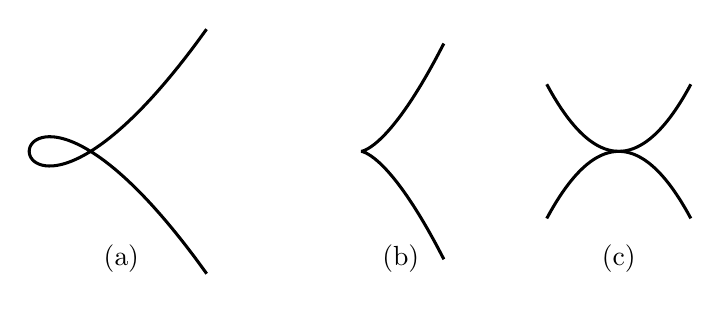
\begin{tikzpicture}[scale=0.78,line width=1.1pt]
  \begin{scope}
    \draw plot[smooth,variable=\t,domain=-1.7:1.7,samples=61]
      ({\t*\t-1},{0.62*(\t*\t*\t-\t)});
    \node at (0.5,-1.75) {(a)};
  \end{scope}
  \begin{scope}[xshift=4.4cm]
    \draw plot[smooth,variable=\t,domain=-1.3:1.3,samples=41]
      ({0.8*\t*\t},{0.8*\t*\t*\t});
    \node at (0.65,-1.75) {(b)};
  \end{scope}
  \begin{scope}[xshift=8.6cm]
    \draw plot[smooth,variable=\x,domain=-1.02:1.02,samples=41]
      ({1.15*\x},{1.05*\x*\x});
    \draw plot[smooth,variable=\x,domain=-1.02:1.02,samples=41]
      ({1.15*\x},{-1.05*\x*\x});
    \node at (0,-1.75) {(c)};
  \end{scope}
\end{tikzpicture}
\caption{平面曲线奇点。（依原书手绘图重绘。）}\label{fig:plane-curve-singularities}
\end{figure}

\textbf{13.3.2.}\ \emph{\trhRemark{}。}\quad 关于\trNode、\trCusp{}与\trTacnode，有几种可能的定义。当 $k=\overline{k}$ 时，一个合理的定义如下。设 $C$ 具\trPureDimension{} $1$，而 $p\in C$ 是一个\trClosedPoint。令 $(A,\mathfrak{m})$ 为\trLocalRing{} $\OO_{C,p}$，于是 $A/\mathfrak{m}=k$。我们称 $p$ 是 $C$ 的一个\textbf{\trNode}，若 $\dim_k\mathfrak{m}/\mathfrak{m}^2=2$，且
\[
\operatorname{Sym}^2(\mathfrak{m}/\mathfrak{m}^2)\longrightarrow\mathfrak{m}^2/\mathfrak{m}^3
\]
的\trKernel{}维数为 $1$，并且该\trKernel{}不由 $\mathfrak{m}/\mathfrak{m}^2$ 中某个元素的平方张成。这个定义我们用不到，所以你无须记住它。但你能弄明白它为什么合理吗？你能为\trCusp{}猜出一个合理的定义吗？关于\trNode、\trCusp{}及更多的另一些定义，将在 \S28.2 中给出。

\textbf{13.3.G.（练习）}\quad 证明：扭曲三次曲线 $\Proj k[w,x,y,z]/(wz-xy,\ wy-x^2,\ xz-y^2)$ 是光滑的。（你可以利用它与 $\mathbb{P}^1$ \trIsomorphic{}这一事实来做。但请用这些显式方程来做，以资练习。扭曲三次曲线定义于\mbox{练习~9.3.A}。）

\textbf{13.3.3.}\ \emph{\trTangentPlane{}与\trTangentLine。}\quad 设概形 $X\subset\mathbb{A}^n$ 由方程 $f_1,\dots,f_r$ 切出，而 $X$ 在 $k$-值点 $a=(a_1,\dots,a_n)$ 处是（纯）维数 $d$ 的光滑概形。那么\textbf{$X$ 在 $a$ 处的切 $d$-平面}（tangent $d$-plane to $X$ at $a$；有时记作 $T_aX$）便由 $r$ 条方程
\[
\biggl(\frac{\partial f_i}{\partial x_1}(a)\biggr)(x_1-a_1)+\cdots+\biggl(\frac{\partial f_i}{\partial x_n}(a)\biggr)(x_n-a_n)=0,
\]
给出，其中（如 \eqref{eq:jacobian-corank-matrix} 中那样）$\frac{\partial f_i}{\partial x_1}(a)$ 表示 $\frac{\partial f_i}{\partial x_1}$ 在 $a=(a_1,\dots,a_n)$ 处的取值。

\textbf{13.3.H.（练习）}\quad 为什么这与 $X$ 的定义方程 $f_1,\dots,f_r$ 的\emph{选取}无关？

\trRegularity{}的\trJacobianCriterion（\mbox{练习~13.2.E}）保证这 $r$ 条方程确实切出一个 $d$-平面。（当 $d=1$ 时，它称为\trTangentLine。）不难证明：这正是我们在多元微积分中所见到的那种\trTangentPlane{}观念\footnote{原书此处作（can be readily shown to be notion of tangent plane），当脱一「the」，径补。——译者注}。但请注意，在这里它是\emph{定义}，因此我们不必操心那些 $\delta$ 与 $\epsilon$。我们所需当心的只是：它要按我们期望的方式行事。

\textbf{13.3.I.（练习）}\quad 计算\mbox{练习~13.3.F(b)}的曲线在 $(1,1)$ 处的\trTangentLine。

\textbf{13.3.J.（练习）}\quad 计算\mbox{练习~13.3.G}的扭曲三次曲线在 $[1,1,1,1]$ 处的（射影）\trTangentLine。

\textbf{13.3.K.（练习）}\quad 设 $X\subset\mathbb{P}^n_k$（$k$ 照常是一个域）由\trHomogeneous{}方程 $f_1,\dots,f_r$ 切出，而 $p\in X$ 是一个（纯）维数为 $d$ 的光滑 $k$-值点。定义 $X$ 在 $p$ 处的（射影）切 $d$-平面。（定义~9.3.3 给出了 $\mathbb{P}^n_k$ 中 $d$-平面的定义，但你应当无须去查它。）

\textbf{13.3.4.}\ \emph{帮你把思路理清爽的旁注。}\quad 我们会希望切 $k$-平面的定义是自然的，其含义是：对 $\mathbb{A}^n_k$ 的任何\trAutomorphism{} $\sigma$（或者，在上一道练习的情形，$\mathbb{P}^n_k$ 的任何\trAutomorphism），都有 $\sigma(T_pX)=T_{\sigma(p)}\sigma(X)$。你可以动手直接验证这一点，但你也可以用更清爽的方式来说：以\trCoordinateFree{}的方式解读切出\trTangentSpace{}的那些方程。非正式地说，我们是在使用「$n$ 维空间」与「$n$ 维空间在 $p$ 处的\trTangentSpace」之间的\trCanonical{}等同，并且在利用这样一件事实：雅可比「\trLinearTransformation」切出 $T_p\mathbb{A}^n_k$ 中的 $T_pX$ 的方式，既不依赖于 $\mathbb{A}^n$ 上坐标的选取，也不依赖于我们对 $X$ 的定义方程。你对\mbox{练习~13.3.H}的解答，将有助于你开始以这种方式思考。

\textbf{13.3.L.（练习）}\quad 设 $X\subset\mathbb{P}^n_k$ 是由 $f=0$ 切出的一张次数为 $d$ 的超曲面，而 $L$ 是一条不含于 $X$ 的直线。\mbox{练习~9.3.D}（\trBezout{}定理的一个特例）表明：$X$ 与 $L$ 交于 $d$ 个点，按「重数」计入。设 $L$ 在一个 $k$-值点 $p\in L\cap X$ 处与 $X$ 相交的「重数至少为 $2$」，且 $p$ 是 $X$ 的正则点。证明：$L$ 含于 $X$ 在 $p$ 处的\trTangentPlane。（你的脑海里有一幅这样的图景吗？）

\textbf{13.3.5.}\ \emph{算术例子。}

\textbf{13.3.M.（容易的练习）}\quad 证明：$\Spec\mathbb{Z}$ 是一条正则\trCurve。

\textbf{13.3.N.（练习）}\quad （这道棘手的练习是为那些知道\textbf{\trGauss{}整数}（Gaussian integers）$\mathbb{Z}[i]$ 的诸素元的读者准备的。）证明 $\mathbb{Z}[i]$ 的维数为 $1$，办法有好几种。（例如：（i）它是一个\trPID；（ii）它是 $\mathbb{Z}$ 在域扩张 $\mathbb{Q}(i)/\mathbb{Q}$ 中的\trNormalization；（iii）用\trKrull{}\trPrincipalIdealTheorem~12.3.3 以及「$\dim\mathbb{Z}[x]=2$（\mbox{练习~12.1.I}）」这条事实。）证明：$\Spec\mathbb{Z}[i]$ 是一条正则\trCurve。（有好几条路可走。你可以用\mbox{练习~13.1.B}。作为一道可以先行演练的例子，考虑素理想 $(1+i)$，它在 $\Spec\mathbb{Z}[x]/(x^2+1)$ 中由方程 $1+x$ 切出。）日后（\S13.5.9）讨论了\trDVR{}之后，我们会有更简单的办法。

\textbf{13.3.O.（练习）}\quad 证明：$[(5,5i)]$ 是 $\Spec\mathbb{Z}[5i]$ 的唯一\trSingularPoint。（提示：$\mathbb{Z}[i]_5\cong\mathbb{Z}[5i]_5$。用上一道练习。）

\textbf{13.3.6.}\ \emph{回到几何：$\mathbb{A}^n_k$ 是正则的。}\quad 证明 $\mathbb{A}^n_k$（$k$ 是一个域）正则的关键一步，是下面这条。

\textbf{13.3.7.\ \trhProposition{}。}\ ——\ \emph{设 $(B,\mathfrak{n},k)$ 是维数为 $d$ 的\trRegular\trLocalRing。令 $\phi\colon B\to B[x]$。设 $\mathfrak{p}$ 是 $A:=B[x]$ 的一个\trPrimeIdeal，满足 $\mathfrak{n}B[x]\subset\mathfrak{p}$。那么 $A_{\mathfrak{p}}$ 是\trRegular\trLocalRing。}

\emph{证明。}\ 几何地说：我们有态射 $\pi\colon X=\Spec B[x]\to Y=\Spec B$，且 $\pi([\mathfrak{p}])=[\mathfrak{n}]$。纤维 $\pi^{-1}([\mathfrak{n}])$ 是 $\Spec(B[x]/\mathfrak{n}B[x])=\Spec k[x]$。于是，要么 (i) $[\mathfrak{p}]$ 是 $[\mathfrak{n}]$ 上方的纤维 $\mathbb{A}^1_k$，要么 (ii) $[\mathfrak{p}]$ 是纤维 $\mathbb{A}^1_k$ 的一个\trClosedPoint。（见\cref{fig:spec-bx-fiber}。）

\begin{figure}[htbp]
\centering
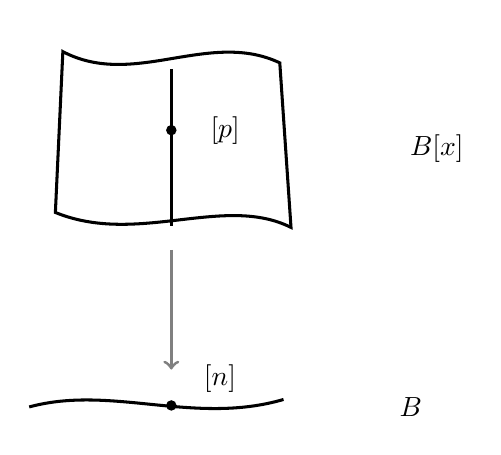
\begin{tikzpicture}[scale=0.95,line width=0.9pt]
  \draw[line width=1.1pt] (-1.55,2.75)
    .. controls (-0.6,2.25) and (0.4,3.05) .. (1.35,2.6)
    -- (1.5,0.4)
    .. controls (0.6,0.85) and (-0.55,0.15) .. (-1.65,0.6)
    -- cycle;
  \draw[line width=1.1pt] (-0.1,2.52) -- (-0.1,0.42);
  \fill (-0.1,1.7) circle (0.07);
  \node at (0.62,1.7) {$[\mathfrak{p}]$};
  \node at (3.45,1.45) {$\Spec B[x]$};
  \draw[gray,line width=1.1pt,->] (-0.1,0.1) -- (-0.1,-1.5);
  \draw[line width=1.1pt] (-2.0,-2.0)
    .. controls (-0.9,-1.7) and (0.2,-2.25) .. (1.4,-1.9);
  \fill (-0.1,-1.98) circle (0.07);
  \node at (0.55,-1.62) {$[\mathfrak{n}]$};
  \node at (3.1,-2.0) {$\Spec B$};
\end{tikzpicture}
\caption{命题~13.3.7 的证明背后的几何。（依原书手绘图重绘。）}\label{fig:spec-bx-fiber}
\end{figure}

在考虑这两种情形之前，我们先作两条注记。由于 $(B,\mathfrak{n})$ 是维数为 $d$ 的\trRegular\trLocalRing，$\mathfrak{n}$ 由 $B$ 的 $d$ 个元素生成，设为 $f_1,\dots,f_d$（\mbox{练习~13.2.D}），并且存在一条素理想链
\begin{equation*}\tag{13.3.7.1}\label{eq:regular-local-prime-chain}
0=\mathfrak{q}_0\subset\mathfrak{q}_1\subset\cdots\subset\mathfrak{q}_d=\mathfrak{n}.
\end{equation*}

\emph{情形 (i)：$[\mathfrak{p}]$ 是纤维 $\mathbb{A}^1_k$。}\ 在此情形，$\mathfrak{p}=\mathfrak{n}B[x]$。于是由\trKrull{}高度定理~12.3.10，$\mathfrak{p}=\mathfrak{n}B[x]$ 的\trCodimension{}至多为 $d$，因为 $\mathfrak{p}$ 由 $d$ 个元素 $f_1,\dots,f_d$ 生成。但 $\mathfrak{p}$ 的\trCodimension{}至少为 $d$：给定以 $\mathfrak{n}$ 收尾的链 \eqref{eq:regular-local-prime-chain}，我们在 $B[x]$ 中便有一条以 $\mathfrak{n}B[x]$ 收尾的相应素理想链。于是 $\mathfrak{p}$ 的\trCodimension{}恰为 $d$，而 $\mathfrak{p}A_{\mathfrak{p}}$ 由 $f_1,\dots,f_d$ 生成，这蕴含它是\trRegular\trLocalRing。

\emph{情形 (ii)：$[\mathfrak{p}]$ 是纤维 $\mathbb{A}^1_k$ 的一个\trClosedPoint。}\ $k[x]$ 的闭点 $\mathfrak{p}$ 对应于某个首一的不可约多项式 $g(x)\in k[x]$。把 $g$ 的系数任意提升到 $B$；我们马虎地把 $B[x]$ 中所得的多项式也记作 $g(x)$。于是 $\mathfrak{p}=(f_1,\dots,f_d,g)$，故由\trKrull{}高度定理~12.3.10，$\mathfrak{p}$ 的\trCodimension{}至多为 $d+1$。但 $\mathfrak{p}$ 的\trCodimension{}至少为 $d+1$：给定以 $\mathfrak{n}$ 收尾的链 \eqref{eq:regular-local-prime-chain}，我们在 $B[x]$ 中便有一条以 $\mathfrak{n}B[x]$ 收尾的相应链，再添上 $\mathfrak{p}$ 即可将其延长。于是 $\mathfrak{p}$ 的\trCodimension{}恰为 $d+1$，而 $\mathfrak{p}A_{\mathfrak{p}}$ 由 $f_1,\dots,f_d,g$ 生成，这蕴含它是\trRegular\trLocalRing。\hfill$\square$

\textbf{13.3.P.（练习）}\quad 用命题~13.3.7 证明：若 $X$ 是正则的（\trLocally\trNoetherian{}的）\trScheme，则 $X\times\mathbb{A}^1$ 亦是。特别地，证明 $\mathbb{A}^n_k$ 是正则的。（提示：想想纤维。）
